\documentclass{beamer}
\usepackage[utf8]{inputenc}
\usepackage{helvet}
\usepackage[english, ngerman]{babel}
\usepackage{hyperref}
\usecolortheme{tum}
\useoutertheme{tum}
\usepackage{xcolor}

\setbeamerfont{author}{size=\footnotesize}
\setbeamerfont{date}{size=\scriptsize}
\setbeamerfont{date}{size=\scriptsize}

\useinnertheme{rectangles}

\usepackage{minted}
\usemintedstyle{vs}

\setminted[haskell]{
    escapeinside=||,
    beameroverlays
}


\usepackage{pgf}
\usepackage{tikz}
\logo{\pgfputat{\pgfxy(-0.2, 8.9)}{\pgfbox[right,top]{
\begin{tikzpicture}[y=0.38pt, x=0.38pt,yscale=-1, inner sep=0pt, outer sep=0pt]
\begin{scope}[cm={{1.25,0.0,0.0,-1.25,(0.0,35.4325)}}]
    \path[fill=tum,nonzero rule] (4.8090,23.2950) -- (4.8090,-0.0020) --
      (9.8590,-0.0020) -- (9.8590,23.2600) -- (15.4730,23.2600) -- (15.4730,-0.0020)
      -- (31.5390,-0.0020) -- (31.5390,23.0140) -- (37.2580,23.0140) --
      (37.2580,0.0060) -- (42.5550,0.0060) -- (42.5550,23.0140) -- (48.3440,23.0140)
      -- (48.3440,0.0060) -- (53.6410,0.0060) -- (53.6410,28.3460) --
      (26.4530,28.3460) -- (26.4530,5.1580) -- (20.6290,5.1580) -- (20.6290,28.3110)
      -- (-0.0000,28.3110) -- (-0.0000,23.2950) -- (4.8090,23.2950) -- cycle;
\end{scope}
\end{tikzpicture}
}}}

\setbeamertemplate{title page}
{
	\vbox{}
	\vfill
	\begin{flushleft}
		\begin{beamercolorbox}[sep=8pt,left]{title}
			\usebeamerfont{title}\inserttitle\par%
			\ifx\insertsubtitle\@empty%
			\else%
				\vskip0.25em%
				{\usebeamerfont{subtitle}\usebeamercolor[fg]{subtitle}\insertsubtitle\par}%
			\fi%
    	\end{beamercolorbox}%
    	\vskip1em\par
		\begin{beamercolorbox}[sep=8pt,left]{author}
		\usebeamerfont{author}\insertauthor
		\end{beamercolorbox}
		\begin{beamercolorbox}[sep=8pt,left]{institute}
		\usebeamerfont{institute}\insertinstitute
		\end{beamercolorbox}
		\begin{beamercolorbox}[sep=8pt,left]{date}
		\usebeamerfont{date}\insertdate
		\end{beamercolorbox}\vskip0.5em
		{\usebeamercolor[fg]{titlegraphic}\inserttitlegraphic\par}
	\end{flushleft}
	\vfill
}

\mode<presentation>

\title{Theorem Proving for All: Equational Reasoning in Liquid Haskell}
\subtitle{\cite{tpfa}}

\author{Jan van Brügge}

\begin{document}

\begin{frame}
\titlepage
\end{frame}

\begin{frame}[fragile]
\frametitle{Equational reasoning}

\begin{minted}{haskell}
fact :: Int -> Int
fact 0 = 1
fact n = n * fact (n - 1)
\end{minted}

\pause

\vspace{10pt}

\begin{minted}{haskell}
let x = fact 3|\pause|
      = 3 * fact (3 - 1)|\pause|
      = 3 * fact 2|\pause|
      = 3 * (2 * fact (2 - 1))|\pause|
      = {- ... -}
      = 3 * (2 * (1 * fact 0))|\pause|
      = 3 * (2 * (1 * 1))|\pause|
      = 6
\end{minted}

\end{frame}

\begin{frame}[fragile]
\frametitle{LiquidHaskell}

\begin{onlyenv}<1>
\begin{minted}{haskell}
fact :: Int -> Int
fact 0 = 1
fact n = n * fact (n - 1)
\end{minted}
\end{onlyenv}

\begin{onlyenv}<2>
\begin{minted}{haskell}
{-@ fact :: { x:Int | x >= 0 } -> Int @-}
fact :: Int -> Int
fact 0 = 1
fact n = n * fact (n - 1)
\end{minted}
\end{onlyenv}

\begin{onlyenv}<3>
\begin{minted}{haskell}
{-@ fact :: { x:Int | x >= 0 } -> { y:Int | y >= 0 } @-}
fact :: Int -> Int
fact 0 = 1
fact n = n * fact (n - 1)
\end{minted}
\end{onlyenv}

\begin{onlyenv}<4,6>
\begin{minted}{haskell}
{-@ type Nat = { x:Int | x >= 0 } @-}

{-@ fact :: Nat -> Nat @-}
fact :: Int -> Int
fact 0 = 1
fact n = n * fact (n - 1)
\end{minted}
\end{onlyenv}

\begin{onlyenv}<5>
\begin{minted}{haskell}
{-@ type Nat = { x:Int | x >= 0 } @-}
type Nat = Int

{-@ fact :: Nat -> Nat @-}
fact :: Nat -> Nat
fact 0 = 1
fact n = n * fact (n - 1)
\end{minted}
\end{onlyenv}

\end{frame}

\begin{frame}[fragile]
\frametitle{Lightweight vs Deep reasoning}

\begin{onlyenv}<1>
\begin{minted}{haskell}
head :: [a] -> a
head [] = error "impossible"
head (x:_) = x
\end{minted}
\end{onlyenv}

\begin{onlyenv}<2>
\begin{minted}{haskell}
{-@ head :: { xs:[a] | ??? } -> a @-}
head :: [a] -> a
head [] = error "impossible"
head (x:_) = x
\end{minted}
\end{onlyenv}

\begin{onlyenv}<3>
\begin{minted}{haskell}
{-@ head :: { xs:[a] | ??? } -> a @-}
head :: [a] -> a
head [] = error "impossible"
head (x:_) = x
\end{minted}

\vspace{10pt}
Measures:
\begin{itemize}
\item{single argument}
\item{which is an algebraic data type}
\item{returns a numeric type}
\item{one equation per constructor}
\item{only uses arithmetic and other measures}
\end{itemize}
\end{onlyenv}

\begin{onlyenv}<4>
\begin{minted}{haskell}
{-@ measure length @-}
{-@ length :: [a] -> Nat @-}
length :: [a] -> Int
length [] = 0
length (_:xs) = 1 + length xs
\end{minted}

\vspace{10pt}

Measures:
\begin{itemize}
\item{single argument}
\item{which is an algebraic data type}
\item{returns a numeric type}
\item{one equation per constructor}
\item{only uses arithmetic and other measures}
\end{itemize}

\end{onlyenv}

\begin{onlyenv}<5>
\begin{minted}{haskell}
{-@ head :: { xs:[a] | length xs > 0 } -> a @-}
head :: [a] -> a
head [] = error "impossible"
head (x:_) = x
\end{minted}
\end{onlyenv}

\begin{onlyenv}<6>
\begin{minted}{haskell}
{-@ head :: { xs:[a] | length xs > 0 } -> a @-}
head :: [a] -> a
head [] = error "impossible"
head (x:_) = x

{-@ (++) :: xs:[a] -> ys:[a] ->
    { zs:[a] | length zs == length xs + length ys } @-}
(++) :: [a] -> [a] -> [a]
[]     ++ ys = ys
(x:xs) ++ ys = x:(xs ++ ys)
\end{minted}
\end{onlyenv}

\end{frame}

\begin{frame}[fragile]
\frametitle{Proof combinators}

\begin{minted}{haskell}
infixl 3 ===
{-@ (===) :: x:a -> { y:a | y == x } ->
    { z:a | z == x && z == y } @-}
(===) :: a -> a -> a
_ === y = y
|\pause|
type Proof = ()
|\pause|
infixl 3 ***
{-@ assume (***) :: a -> p:QED ->
    { if (isAdmit p) then false else true } @-}
(***) :: a -> QED -> Proof
_ *** _ = ()
data QED = Admit | QED
{-@ measure isAdmit :: QED -> Bool @-}
{-@ Admit :: {v:QED | isAdmit v } @-}
\end{minted}


\end{frame}

\begin{frame}[fragile]
\frametitle{Deriving efficient implementations from simple specifications}

\begin{onlyenv}<1>
\begin{minted}{haskell}
{-@ reverse :: xs:[a] ->
    { ys:[a] | length xs == length ys } @-}
reverse [] = []
reverse (x:xs) = reverse xs ++ [x]
\end{minted}
\end{onlyenv}

\begin{onlyenv}<2>
\begin{minted}{haskell}
{-@ reverse :: xs:[a] ->
    { ys:[a] | length xs == length ys } @-}
reverse [] = []
reverse (x:xs) = reverse xs ++ [x]

{-@ reflect (++) @-}
{-@ reflect reverse @-}

{-@ revApp :: xs:[a] -> ys:[a] ->
    { zs:[a] | revApp xs ys == reverse xs ++ ys } @-}
revApp :: [a] -> [a] -> [a]
revApp xs ys = undefined
\end{minted}
\end{onlyenv}

\begin{onlyenv}<3>
\begin{minted}{haskell}
{-@ revApp :: xs:[a] -> ys:[a] ->
    { zs:[a] | revApp xs ys == reverse xs ++ ys } @-}
revApp :: [a] -> [a] -> [a]
revApp xs ys = reverse xs ++ ys
\end{minted}
\end{onlyenv}

\begin{onlyenv}<4>
\begin{minted}{haskell}
{-@ revApp :: xs:[a] -> ys:[a] ->
    { zs:[a] | revApp xs ys == reverse xs ++ ys } @-}
revApp :: [a] -> [a] -> [a]
revApp [] ys = reverse [] ++ ys
revApp (x:xs) ys = reverse (x:xs) ++ ys
\end{minted}
\end{onlyenv}

\begin{onlyenv}<5>
\begin{minted}{haskell}
{-@ revApp :: xs:[a] -> ys:[a] ->
    { zs:[a] | revApp xs ys == reverse xs ++ ys } @-}
revApp :: [a] -> [a] -> [a]
revApp [] ys = reverse [] ++ ys
    === [] ++ ys
    === ys
revApp (x:xs) ys = reverse (x:xs) ++ ys
\end{minted}
\end{onlyenv}

\begin{onlyenv}<6>
\begin{minted}{haskell}
{-@ revApp :: xs:[a] -> ys:[a] ->
    { zs:[a] | revApp xs ys == reverse xs ++ ys } @-}
revApp :: [a] -> [a] -> [a]
revApp [] ys = reverse [] ++ ys
    === [] ++ ys
    === ys
revApp (x:xs) ys = reverse (x:xs) ++ ys
    === (reverse xs ++ [x]) ++ ys
\end{minted}
\end{onlyenv}

\begin{onlyenv}<7>
\begin{minted}{haskell}
{-@ apAssocP :: xs:[a] -> ys:[a] -> zs:[a] ->
    { (xs ++ ys) ++ zs == xs ++ (ys ++ zs) } @-}
apAssocP :: [a] -> [a] -> [a] -> Proof
apAssocP xs ys zs = undefined
\end{minted}
\end{onlyenv}

\begin{onlyenv}<8>
\begin{minted}{haskell}
{-@ apAssocP :: xs:[a] -> ys:[a] -> zs:[a] ->
    { (xs ++ ys) ++ zs == xs ++ (ys ++ zs) } @-}
apAssocP :: [a] -> [a] -> [a] -> Proof
apAssocP [] ys zs = ([] ++ ys) ++ zs
apAssocP (x:xs) ys zs = undefined
\end{minted}
\end{onlyenv}

\begin{onlyenv}<9>
\begin{minted}{haskell}
{-@ apAssocP :: xs:[a] -> ys:[a] -> zs:[a] ->
    { (xs ++ ys) ++ zs == xs ++ (ys ++ zs) } @-}
apAssocP :: [a] -> [a] -> [a] -> Proof
apAssocP [] ys zs = ([] ++ ys) ++ zs
    === ys ++ zs
    === [] ++ (ys ++ zs)
    *** QED
apAssocP (x:xs) ys zs = undefined
\end{minted}
\end{onlyenv}

\begin{onlyenv}<10>
\begin{minted}{haskell}
{-@ apAssocP :: xs:[a] -> ys:[a] -> zs:[a] ->
    { (xs ++ ys) ++ zs == xs ++ (ys ++ zs) } @-}
apAssocP :: [a] -> [a] -> [a] -> Proof
apAssocP [] ys zs = ([] ++ ys) ++ zs
    === ys ++ zs
    === [] ++ (ys ++ zs)
    *** QED
apAssocP (x:xs) ys zs = ((x:xs) ++ ys) ++ zs
    === (x:(xs ++ ys)) ++ zs
    === x:((xs ++ ys) ++ zs)
\end{minted}
\end{onlyenv}

\begin{onlyenv}<11>
\begin{minted}{haskell}
{-@ apAssocP :: xs:[a] -> ys:[a] -> zs:[a] ->
    { (xs ++ ys) ++ zs == xs ++ (ys ++ zs) } @-}
apAssocP :: [a] -> [a] -> [a] -> Proof
apAssocP [] ys zs = ([] ++ ys) ++ zs
    === ys ++ zs
    === [] ++ (ys ++ zs)
    *** QED
apAssocP (x:xs) ys zs = ((x:xs) ++ ys) ++ zs
    === (x:(xs ++ ys)) ++ zs
    === x:((xs ++ ys) ++ zs)
    ? apAssocP xs ys zs
    === x:(xs ++ (ys ++ zs))
    === (x:xs) ++ (ys ++ zs)
    *** QED
\end{minted}
\end{onlyenv}

\begin{onlyenv}<12>
\begin{minted}{haskell}
{-@ revApp :: xs:[a] -> ys:[a] ->
    { zs:[a] | revApp xs ys == reverse xs ++ ys } @-}
revApp :: [a] -> [a] -> [a]
revApp [] ys = reverse [] ++ ys
    === [] ++ ys
    === ys
revApp (x:xs) ys = reverse (x:xs) ++ ys
    === (reverse xs ++ [x]) ++ ys
    ? apAssocP (reverse xs) [x] ys
    === reverse xs ++ ([x] ++ ys)
    === reverse xs ++ (x:([] ++ ys))
    === reverse xs ++ (x:ys)
\end{minted}
\end{onlyenv}

\begin{onlyenv}<13>
\begin{minted}{haskell}
{-@ revApp :: xs:[a] -> ys:[a] ->
    { zs:[a] | revApp xs ys == reverse xs ++ ys } @-}
revApp :: [a] -> [a] -> [a]
revApp [] ys = reverse [] ++ ys
    === [] ++ ys
    === ys
revApp (x:xs) ys = reverse (x:xs) ++ ys
    === (reverse xs ++ [x]) ++ ys
    ? apAssocP (reverse xs) [x] ys
    === reverse xs ++ ([x] ++ ys)
    === reverse xs ++ (x:([] ++ ys))
    === reverse xs ++ (x:ys)
    === revApp xs (x:ys)
\end{minted}
\end{onlyenv}

\end{frame}

\begin{frame}[fragile]
\frametitle{Amortized complexity analysis}

\begin{figure}[ht]
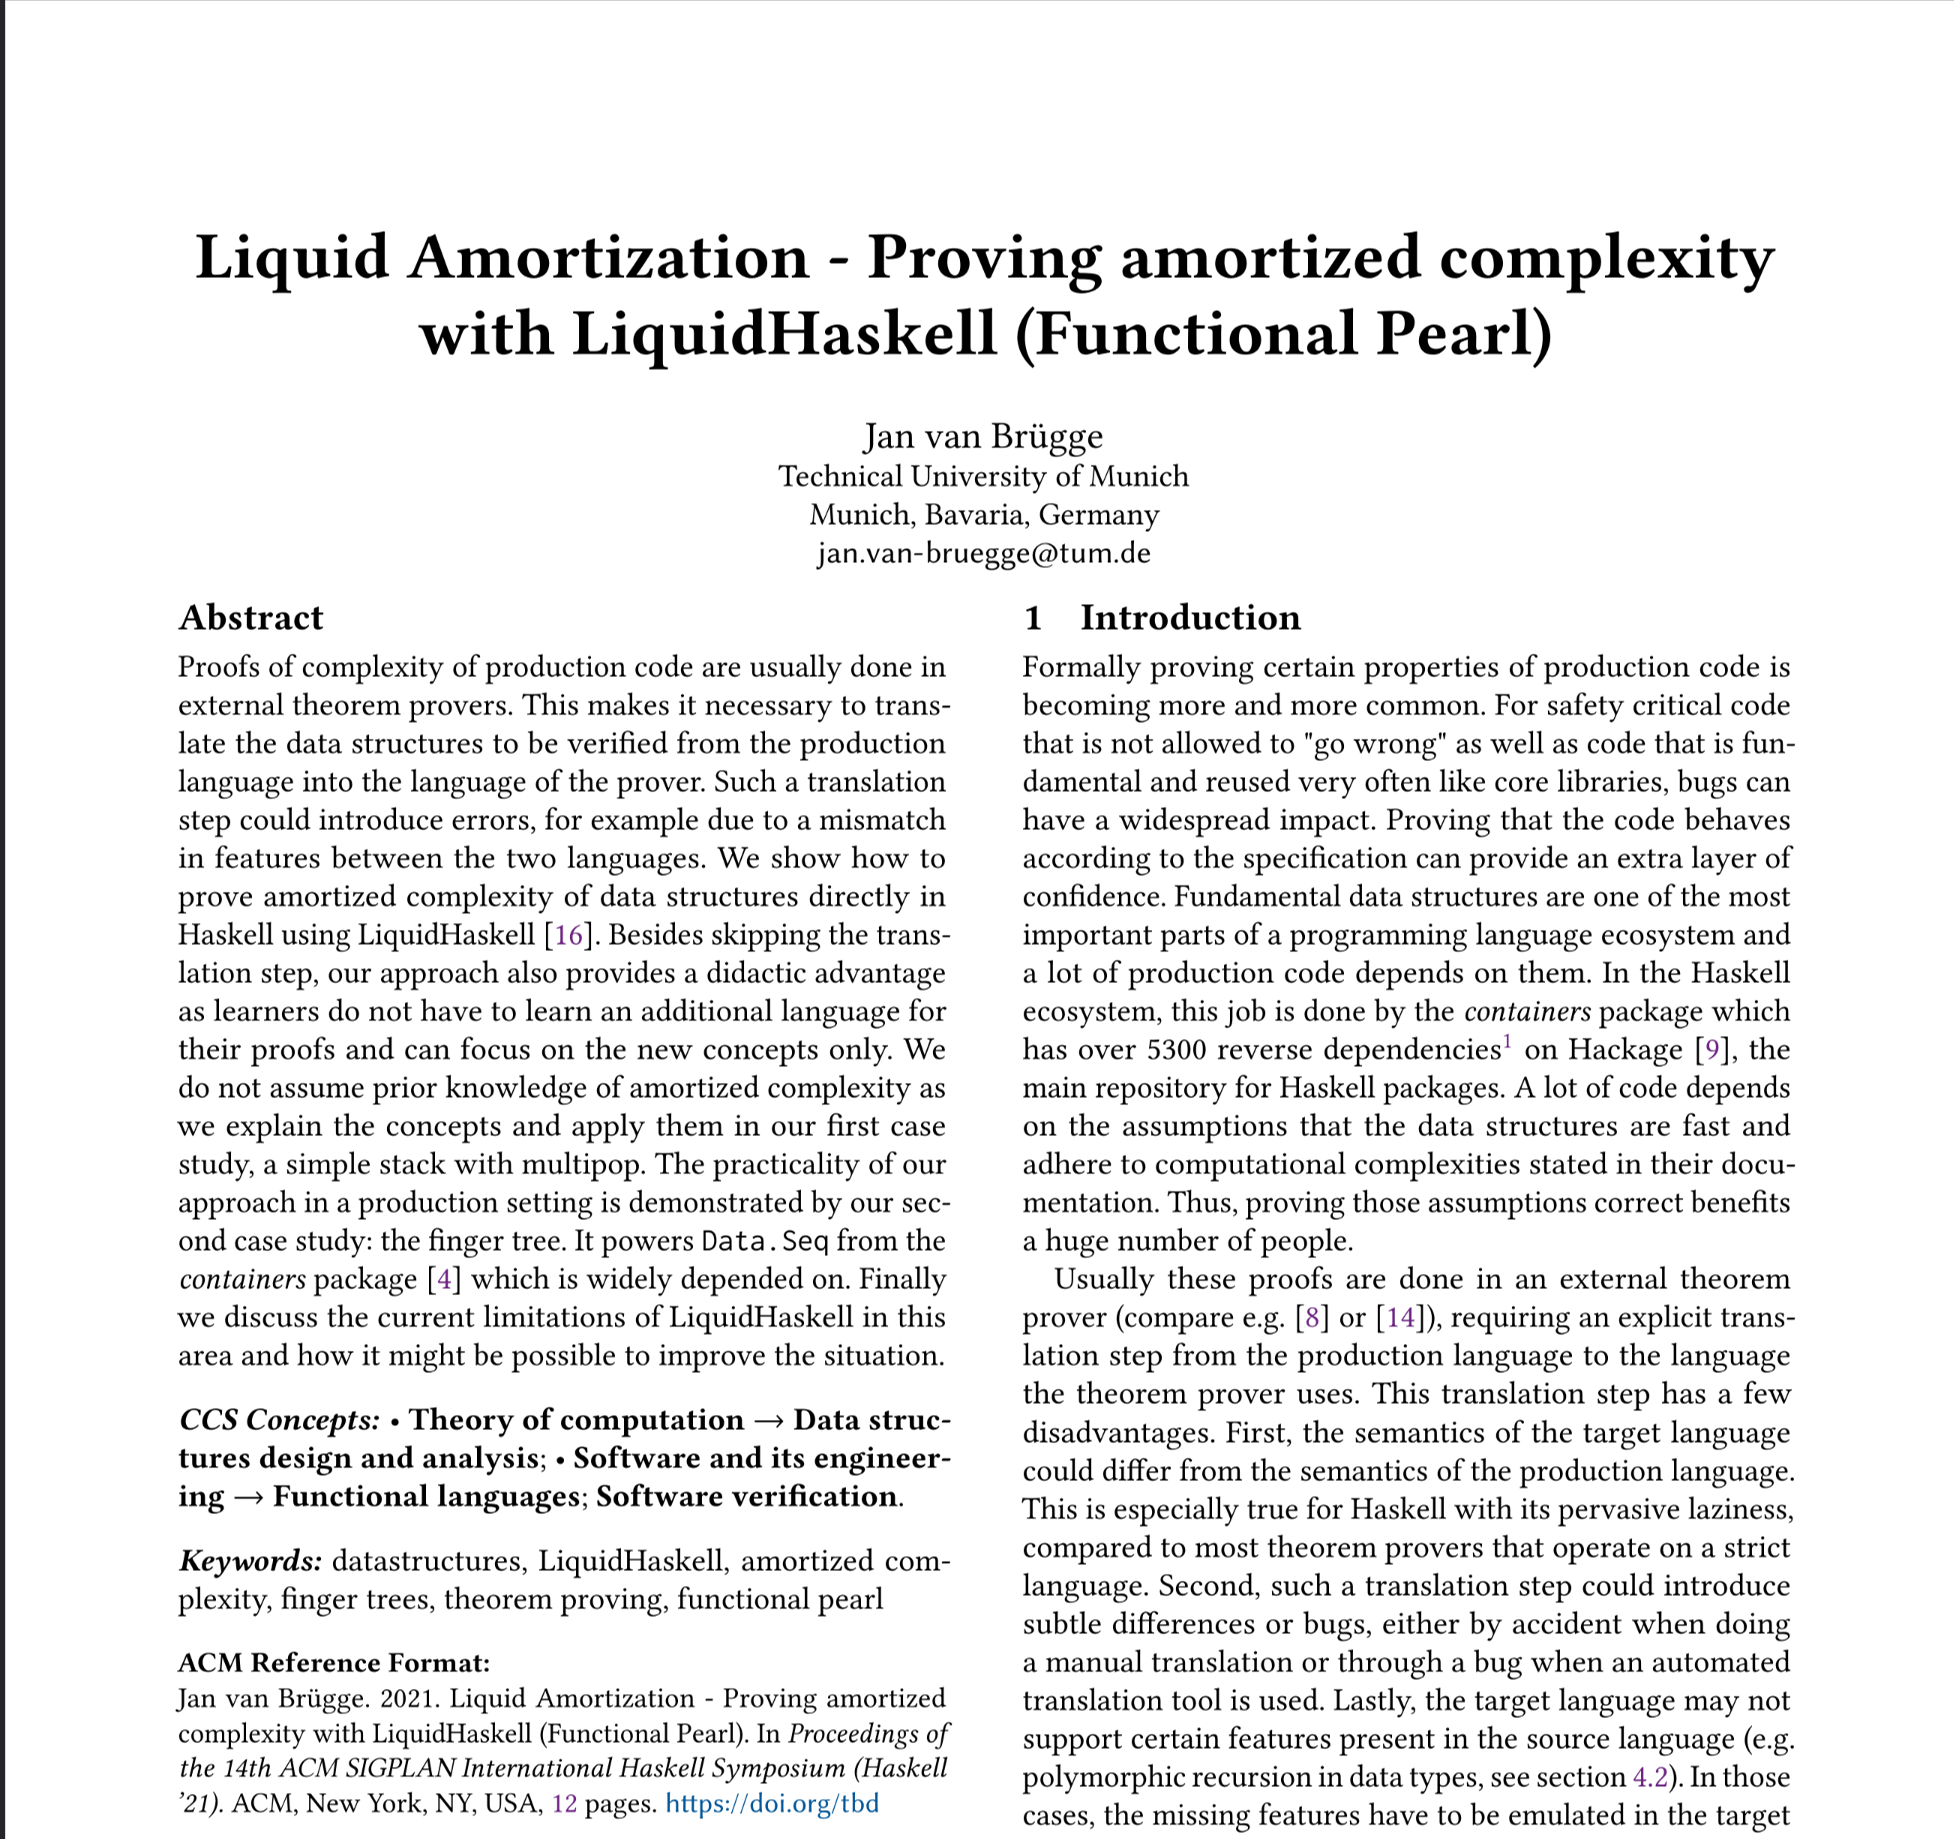
\includegraphics[width=0.7\linewidth,height=0.7\textheight,keepaspectratio]{./paper.png}
\end{figure}

\href{https://github.com/jvanbruegge/liquidhaskell-amortized-complexity/releases/download/v1/liquid_amortization.pdf}{\color{blue}\underline{Available on GitHub}}

\end{frame}

\begin{frame}[fragile]
\frametitle{Limitations}

\begin{itemize}
\item{Combinatorial explosion of constraints}
\pause
\item{Error messages that are hard to understand}
\pause
\item{No real support for type classes:}
\end{itemize}
\begin{minted}{haskell}
class Semigroup a => VSemigroup a where
    {-@ assocP :: x:a -> y:a -> z:a ->
        { (x <> y) <> z == x <> (y <> z) } @-}
    assocP :: a -> a -> a -> Proof
\end{minted}

\end{frame}

\begin{frame}[fragile]
\frametitle{References}

\bibliographystyle{plainnat}
\bibliography{references}

\end{frame}

\end{document}
